\documentclass[a4paper,12pt]{article}

% 导言区
\usepackage{titlesec}
\usepackage{lipsum} % 示例用,可以删除
\usepackage{geometry}
\usepackage{setspace}
\usepackage{amsmath} % 用于数学公式
\usepackage{graphicx} % 用于插入图片
\usepackage{float}
\usepackage{lipsum} % 用于生成虚拟文本
\usepackage{ctex} % 导入 ctex 包以支持中文
\usepackage{titlesec} % 导入 titlesec 包以定制标题样式
\usepackage{fontspec} % 用于设置中文字体
\usepackage{amsfonts}
\usepackage{amsmath} % 提供 \text 和 \tanh 命令
\usepackage{bm}      % 提供 \bm 命令用于粗体
% 目录设置
\usepackage[nottoc,notlot,notlof]{tocbibind}
\usepackage{enumitem}
% 页面设置
\geometry{margin=1in}

% 标题设置
\titleformat{\section}{\normalfont\Large\bfseries}{\thesection}{1em}{}
\titleformat{\subsection}{\normalfont\large\bfseries}{\thesubsection}{1em}{}
\titleformat{\subsubsection}{\normalfont\normalsize\bfseries}{\thesubsubsection}{1em}{}

% 行间距设置
\onehalfspacing

% 文档信息
\title{商业模式评估}
\author{需求不寄小分队}
\date{\today}

\begin{document}

    \maketitle

% 添加目录
    \tableofcontents


    \subsection{团队成员}
    211250124 程智镝

    211250122 刘辉

    211250159 陈凌

    211250158 李忠信
    \subsection{度量数值}

    \section{文档简介}
    

    \section{商业模式环境}
    
    
    \section{商业模式总体评估}
    

    \section{SWOT分析}
    \subsection{S\&W}
    \subsubsection{打分结果}
    \begin{figure}[htbp]
        \centering
        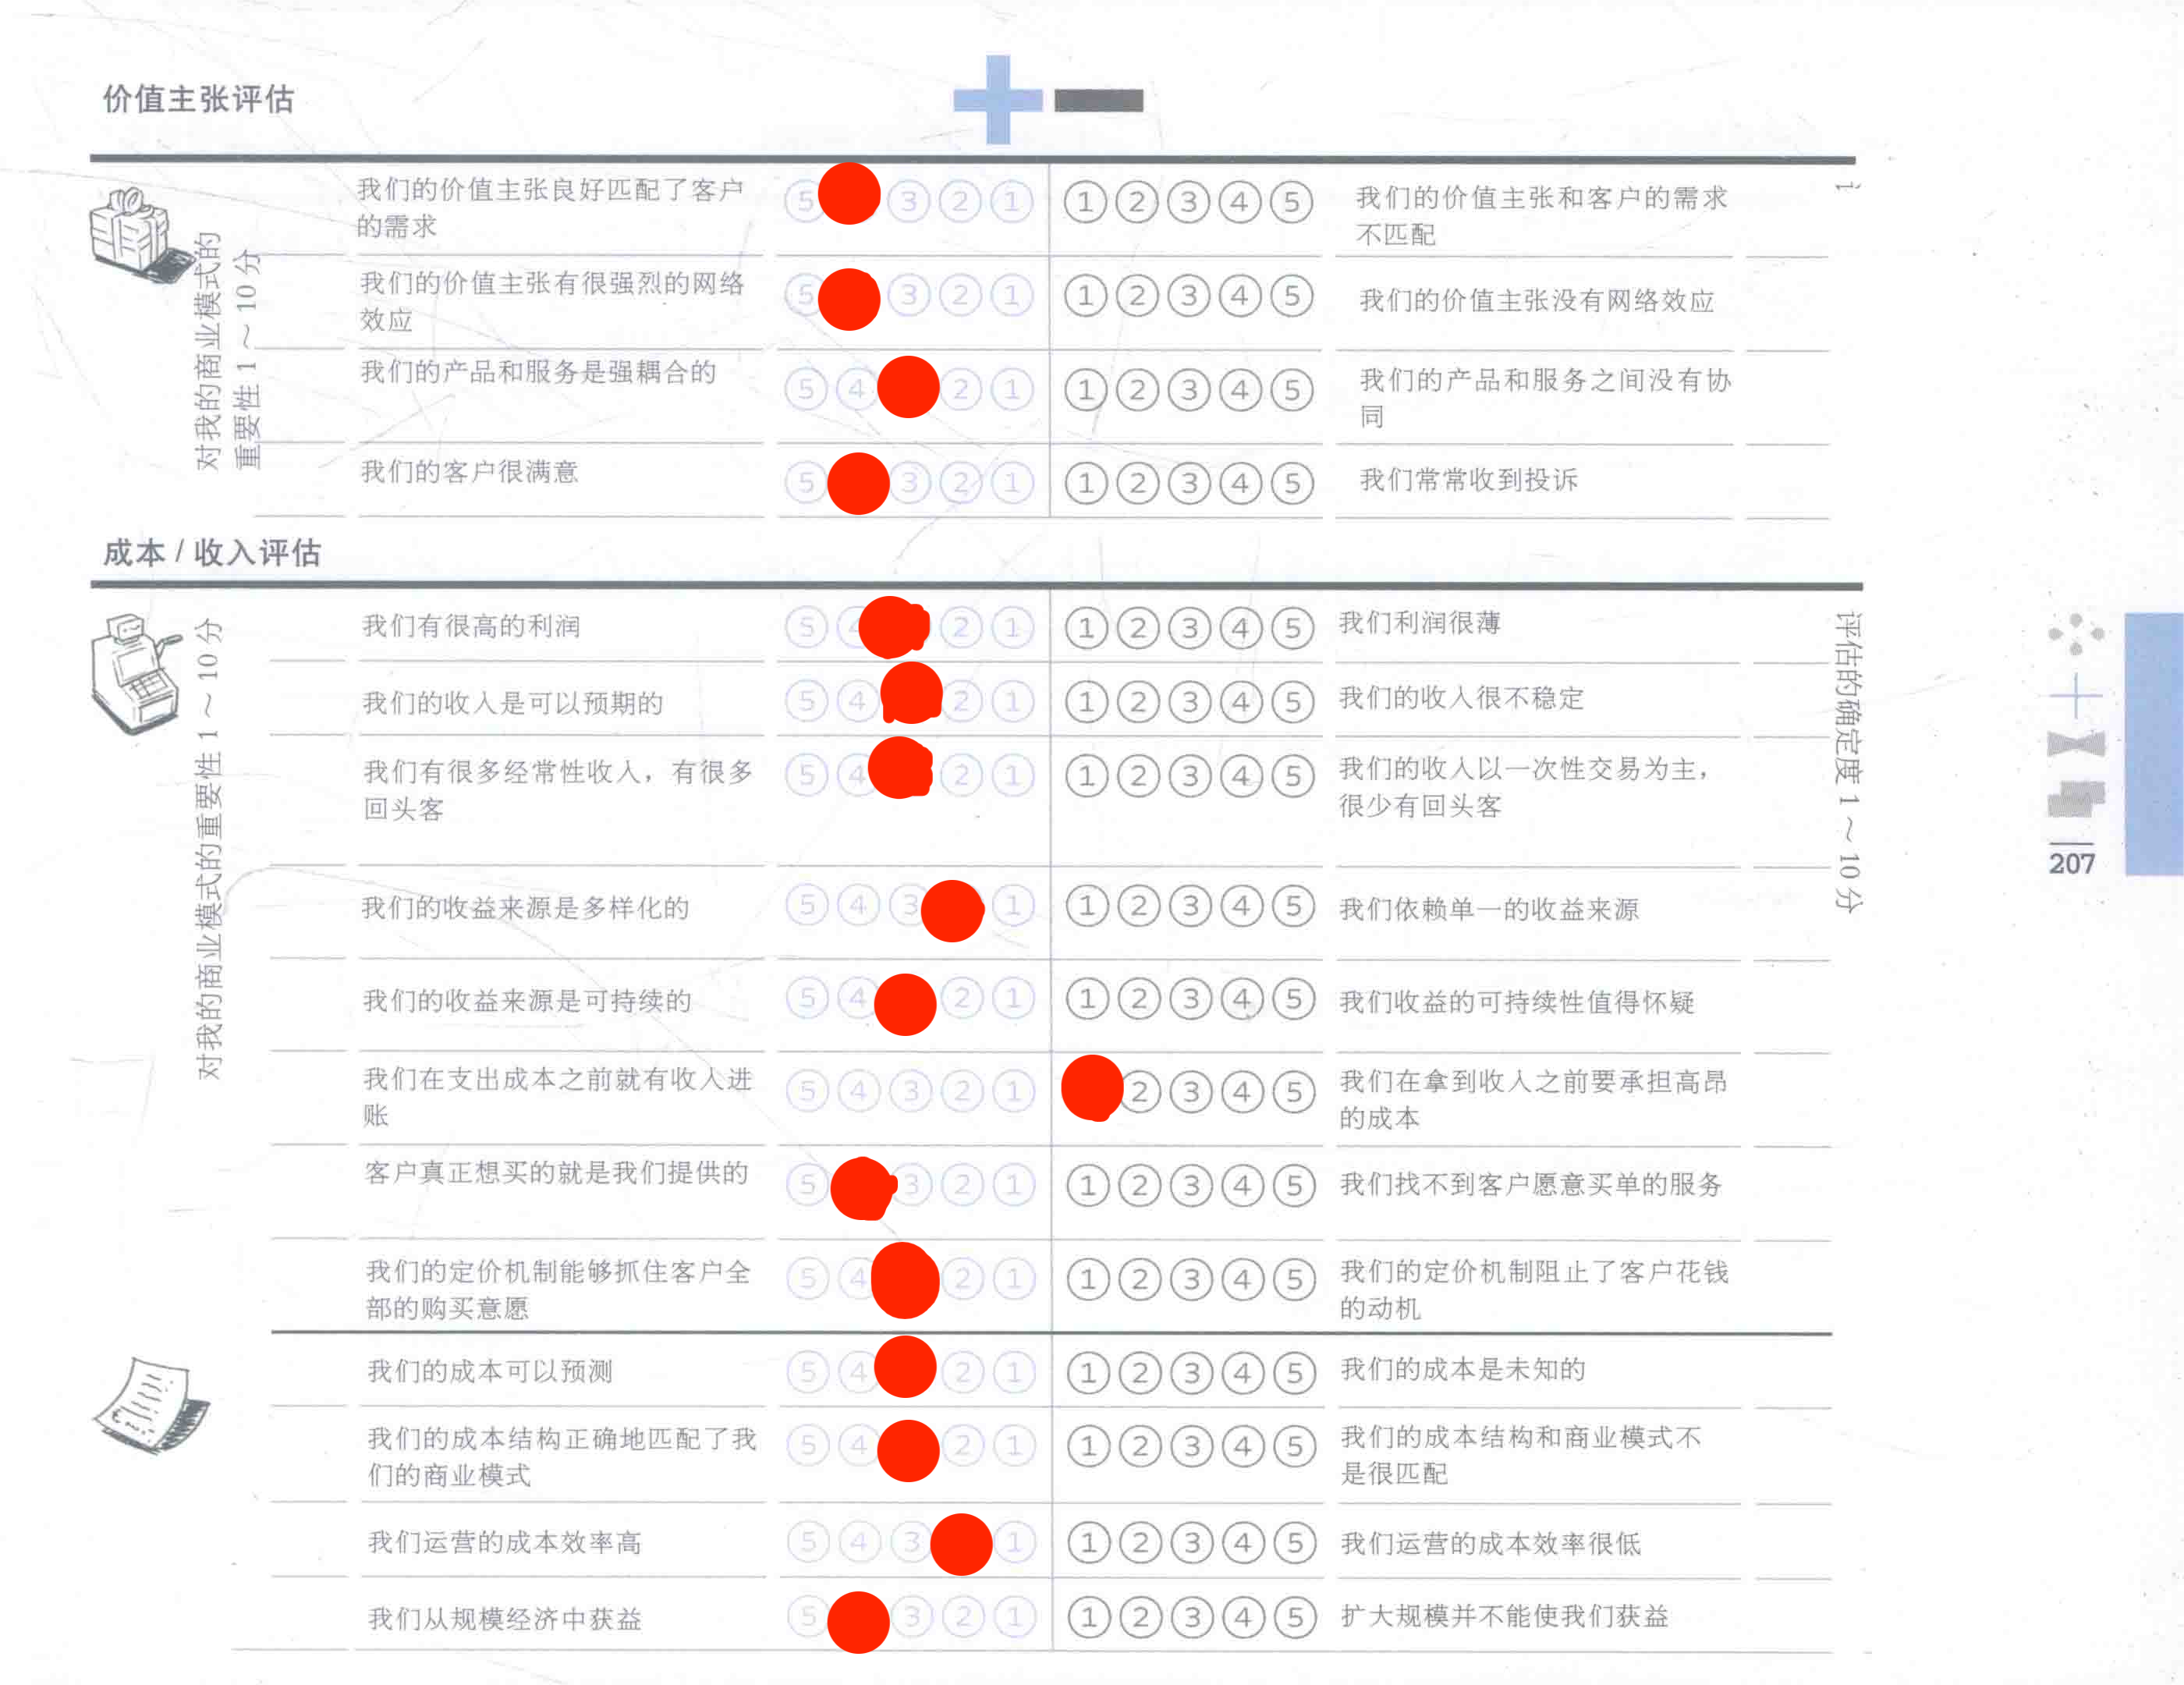
\includegraphics[width=20cm,height=15cm]{png/S&W1}
    \end{figure}
    \begin{figure}[htbp]
        \centering
        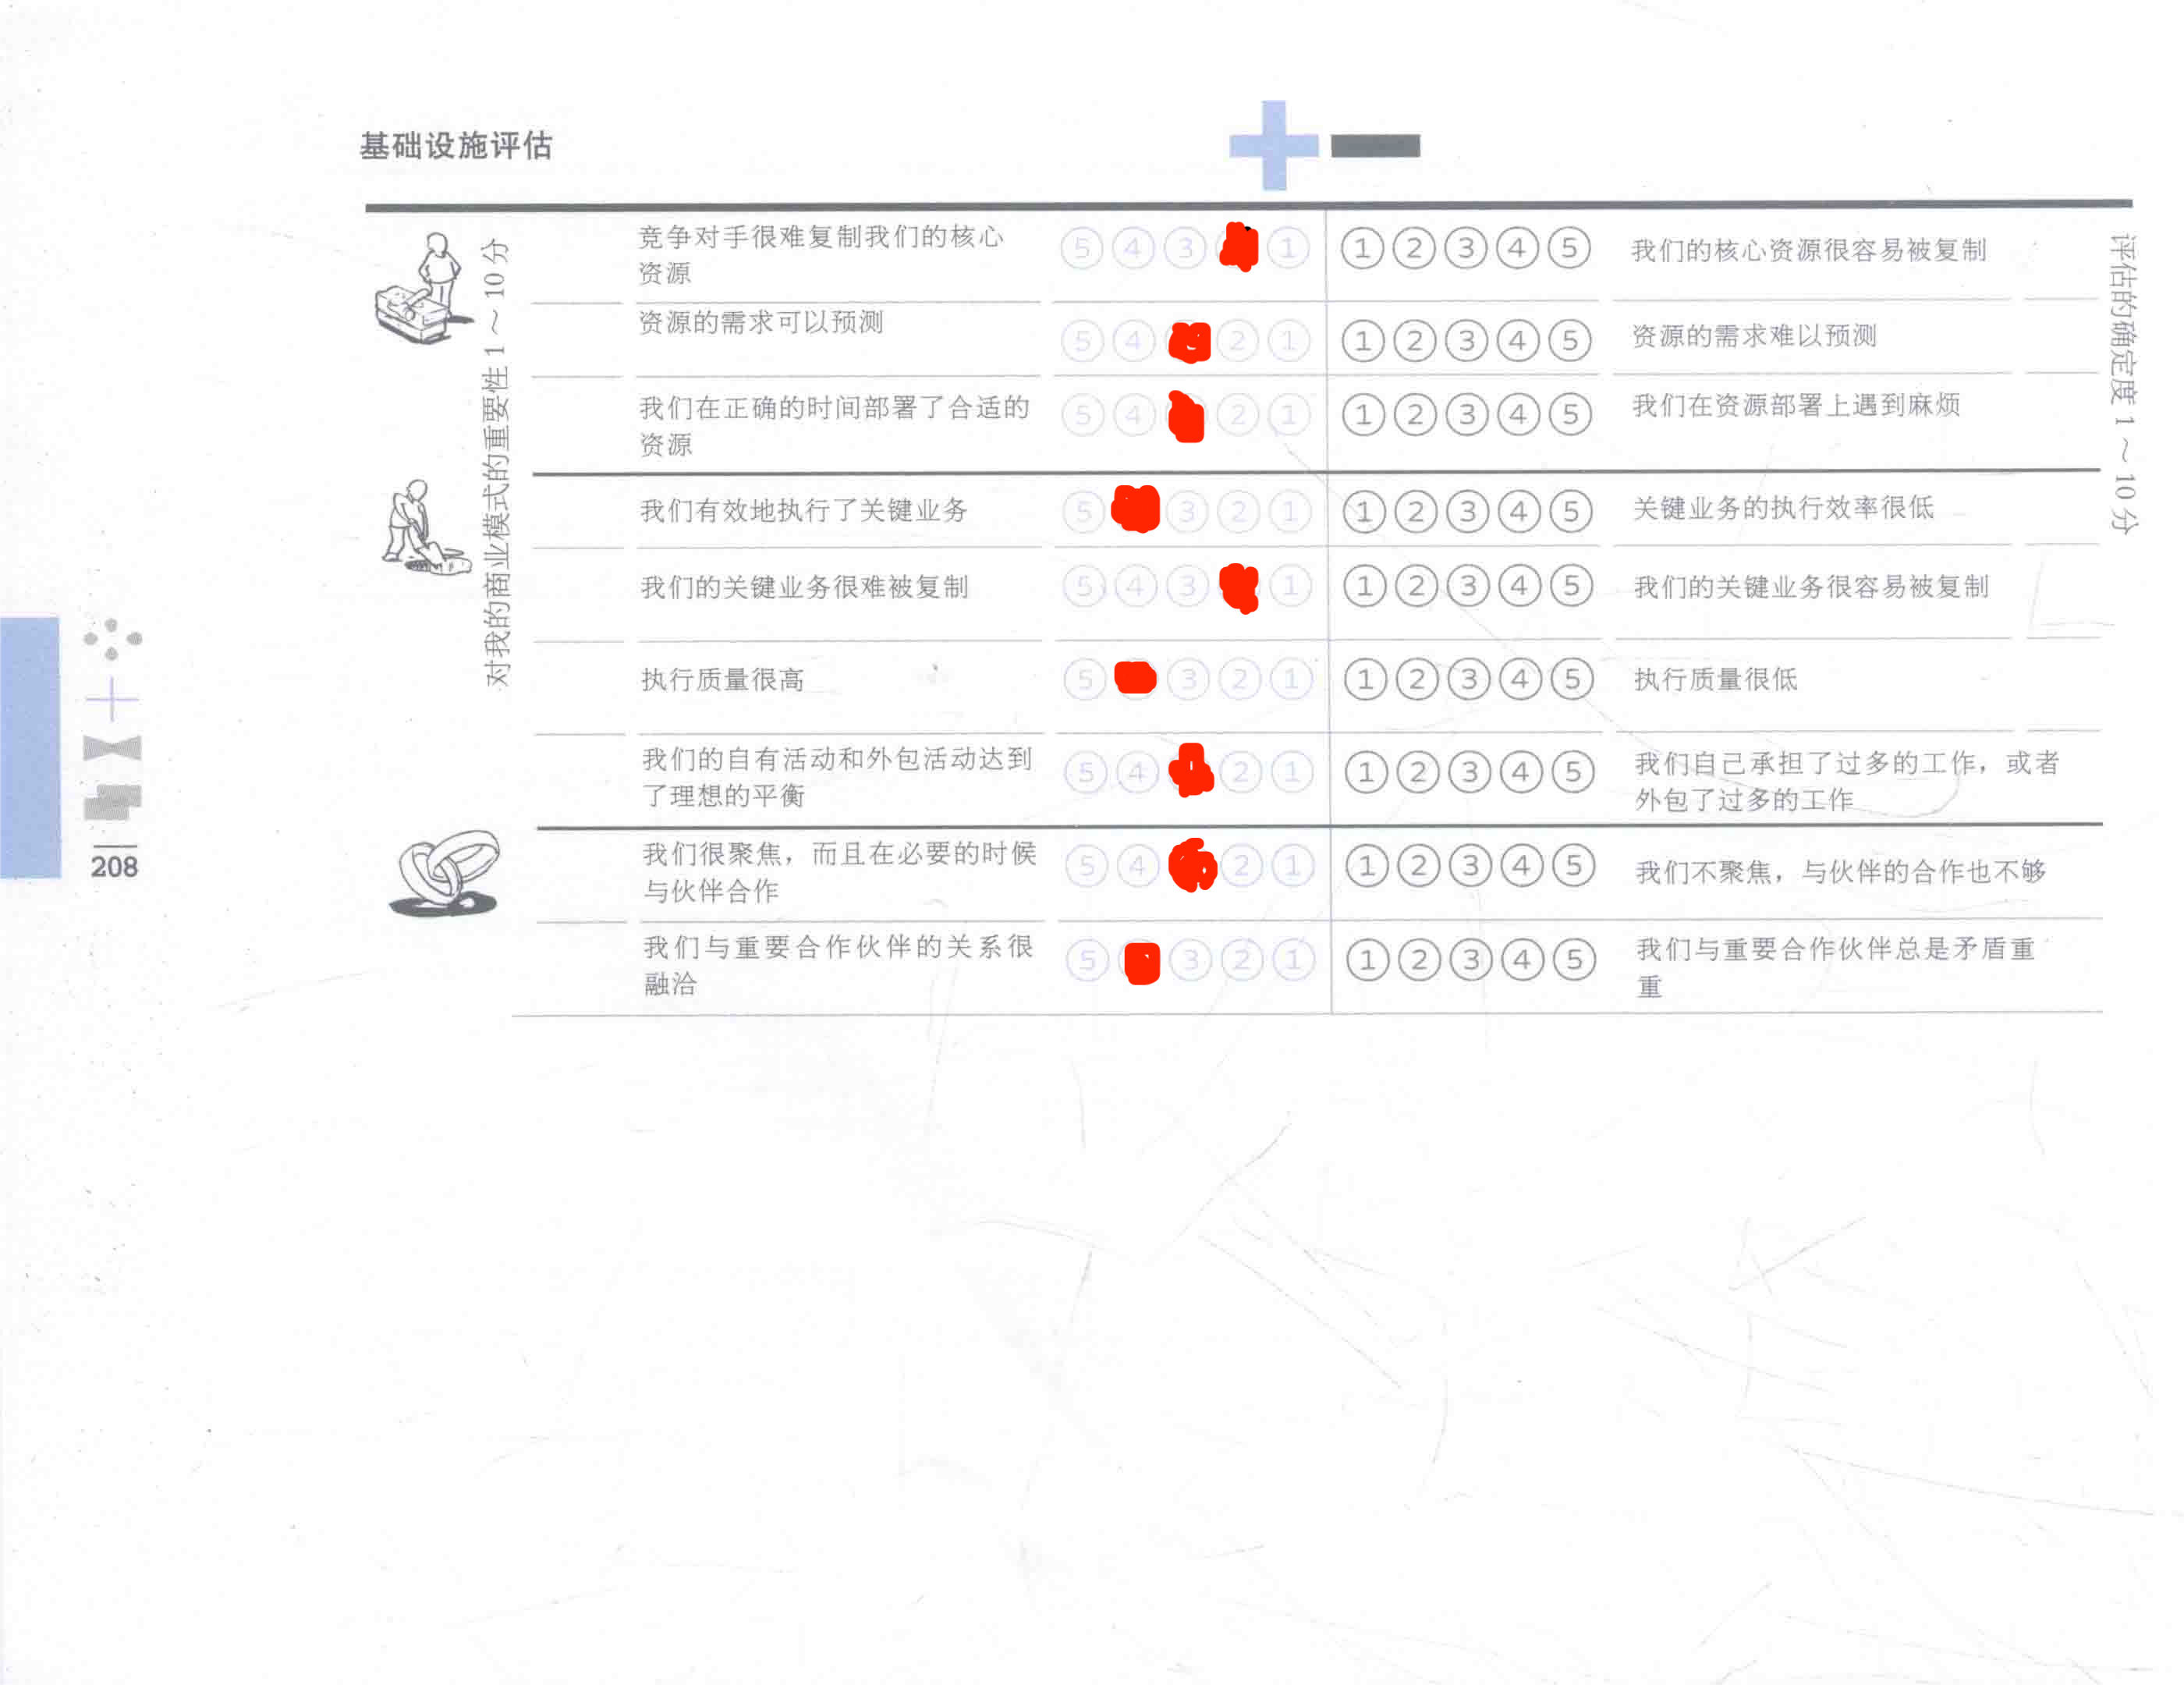
\includegraphics[width=15cm,height=15cm]{png/S&W2}
    \end{figure}
   
    \begin{figure}[htbp]
        \centering
        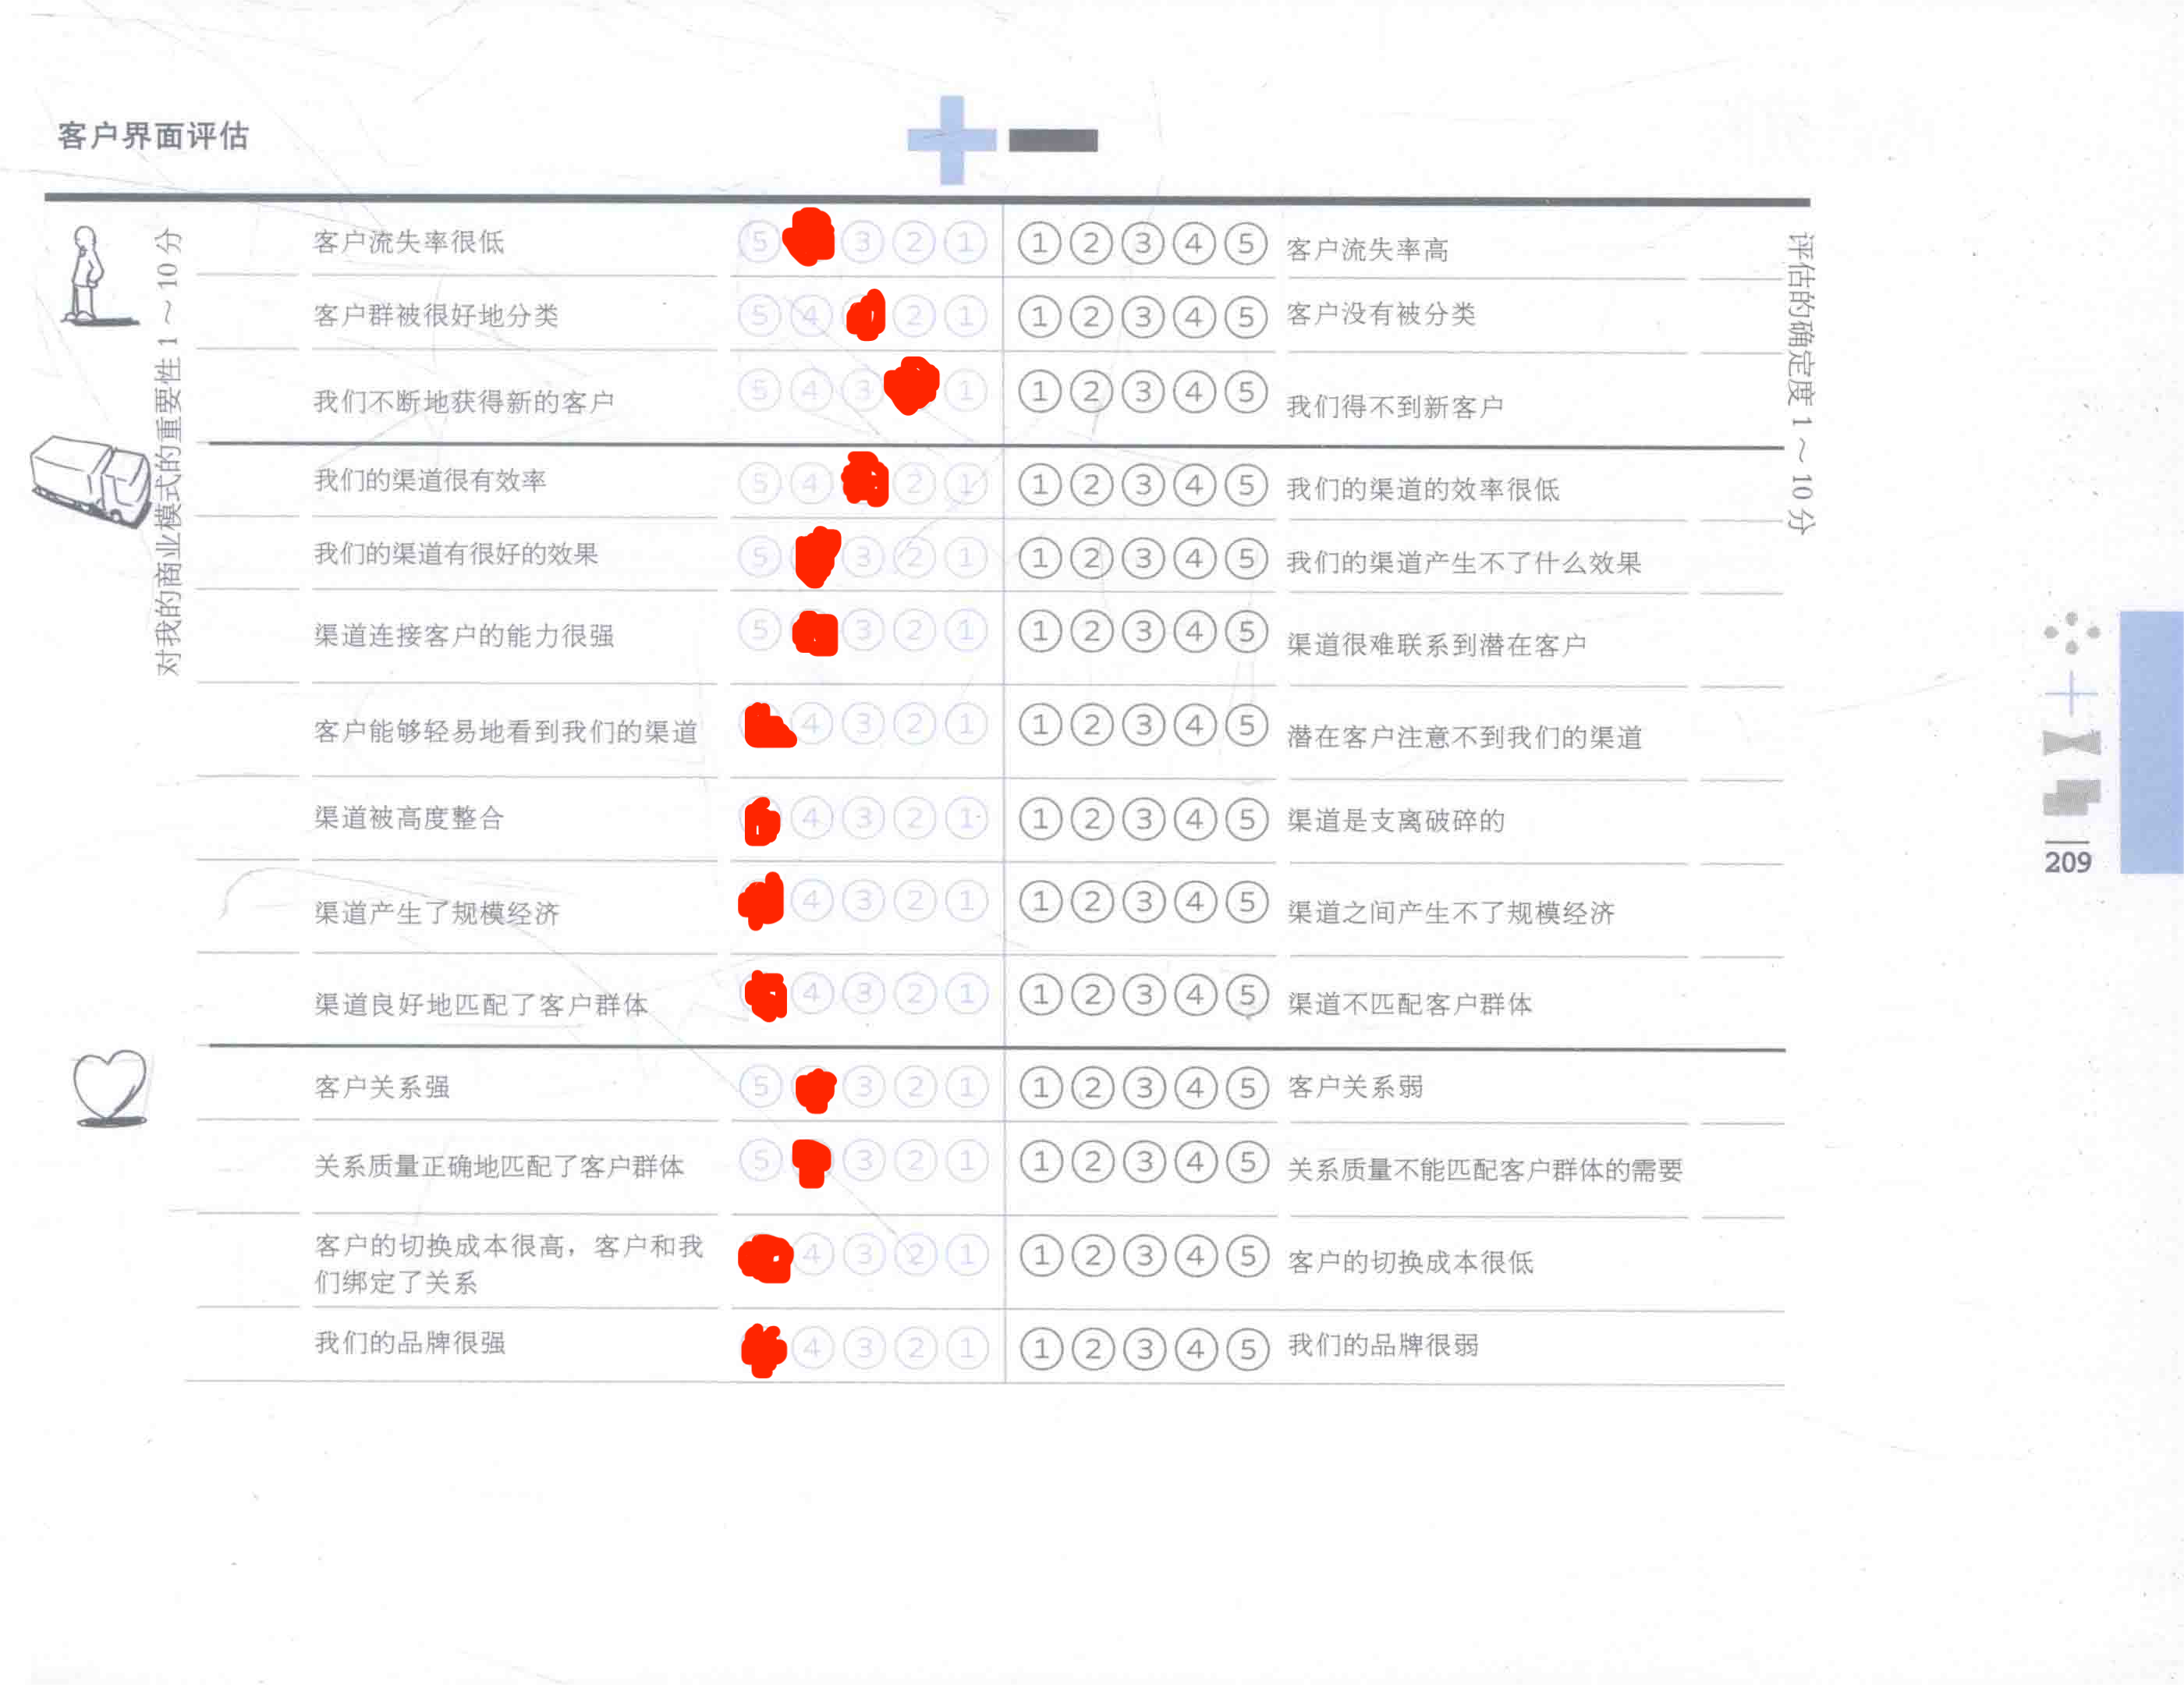
\includegraphics[width=20cm,height=15cm]{png/S&W3}
    \end{figure}
    \clearpage % 强制图片开始新页面
    \subsubsection{价值主张评估}
    \texttt{腾讯会议的独特价值主张}

\begin{itemize}
  \item 腾讯会议产品的价值主张旨在与客户需求紧密契合。他们始终站在客户的角度,深入了解他们真正需要的服务。
  
  \item 提供免费的会议服务,确保普通用户能够轻松享受舒适的会议体验。
  
  \item 为需要更个性化设置、更长时间、更多参会人数以及更大云存储空间等功能的用户提供收费的VIP服务。
  
  \item 面向企业用户提供高级企业会议服务;同时,为学者用户提供专属的“自习室”和网络研讨会议。
  
  \item 始终坚持“对症下药”的原则,以用户为中心,通过收集用户反馈不断优化腾讯会议产品,以满足他们的合理需求。
\end{itemize}

\texttt{腾讯会议的强大网络效应}

\begin{itemize}
  \item 腾讯会议的价值主张具有显著的网络效应。产品的价值取决于使用该产品的其他用户数量,即网络外部性或网络效应。
  
  \item 腾讯会议虚拟会议软件是一个典型的具有网络效应的产品。在刚开始运营时,他们面临高昂的运营成本,并且用户只能与数量有限的人交流信息和使用经验。
  
  \item 随着口碑的积累和知名度的提高,他们将有足够的流水来支付成本并逐渐实现盈利。同时,随着客户数量的增多,像公开会议这种需要大量潜在用户群体的服务也能有效提高腾讯会议产品本身的价值。
  
  \item 因此,腾讯会议的价值主张具有强烈的网络效应。
\end{itemize}

\texttt{腾讯会议的高度耦合产品和服务}

\begin{itemize}
  \item 腾讯会议虚拟会议软件的存在旨在为用户提供仿真实的会议服务。他们追求通过产品为顾客提供最真实、最自然、最愉悦的服务,因此,可以说他们的产品和服务之间存在密切的关系。
\end{itemize}

\texttt{腾讯会议的客户满意度保障}

\begin{itemize}
  \item 他们确信腾讯会议的客户将会非常满意。腾讯会议虚拟会议软件不断追求卓越的用户体验。一旦用户提出不满意的反馈,他们会进行权衡和测试,在经过权衡和测试之后,会做出相应的优化⽅案。
\end{itemize}
\textbf{调研:}
\begin{itemize}
    \item 腾讯会议准备从‘产品的专业能力与体验’进化到‘建设开放生态’,将以更专业、开放的姿态,引入更多的伙伴,更好的服务行业与客户。--《如何理解腾讯会议3.0“会聚力”的价值主张》
    \item 腾讯会议企业版将推出混合云部署,混合云部署更加灵活、稳定,能够方便企业管理员的远程运维,更提高了大型企业的使用感受,内部会议可以部署在专有云上,保证信息资产安全。--《服务3亿用户、14亿场会,腾讯会议企业版迎来重大升级》
    \item 腾讯会议作为在线办公软件中的一匹黑马,自2019年底发布以来就出现了高速增长,仅仅上线两个月内,每日活跃用户就超过1000万,一举成为中国最多视频会议产品,助力全球抗击疫情。--《有人给腾讯会议算了一笔账,5个月节约社会成本高达714亿元》
\end{itemize}
\subsubsection{成本收入评估}
\texttt{腾讯会议较高的利润。}


腾讯会议旗下有众多vip才能享受的服务,这些服务有很多是中大型企业经常甚至必须使用到的,腾讯会议在重视用户体验和口碑的同时,
也会收取相应的费用,对于不经常使用的用户完全可以只使用免费服务即可,腾讯会议的收费功能更多的是面向那些经常要开展大型会议的中大型企业,或者对
线上学术研讨有强烈需求的教育机构等。他们一次会议的人数众多,时间较长,对腾讯会议vip提供的服务有较强的依赖性。他们的vip服务主要分为三个档次:个人会员版、商业版、企业版。针对不同客户都有让他们难以割舍的服务。
腾讯会议的收入基本是可以预期的。在VIP会员费板块,通过引入年卡、连续包月等方式
保证收入的可预期性。同时和教育机构以及高校、企业的合作往往都是长期的,从中收取
的相应的团体专属使用权的购买费用自然是可以预期的。当然,也存在像云存储使用费这
样的可预期性一般的收入,也尽可能的会去通过一次性购买足量的云存储空间给予折
扣的方式来提高其可预期性。\\

\texttt{腾讯会议有很多经常性的收入,有很多回头客的。}腾讯会议提供的VIP服务是具备用户黏性的,他们以用户为中心的主旨会使他们在留住用户这一块有着较强的自信,再加上引入的连续包
月的机制,可以保证收入的经常性。任何回头客都是建立在产品对自己有足够的吸引力之
上的,不断优化的舒适的使用体验是他们最大的竞争力,也是他们留住用户,并从用户群
体中获得经常性收入的保证。其中的会议字幕翻译、实时转译功能对某些跨国企业有非常大的吸引力。\\

\texttt{腾讯会议收入来源是多样的。}基本的收益包括:从个人VIP用户手中收取的VIP服务费,向教育机构、高校与企业收取相应的团体专属使用权的购
买费用,对有拥有更大的云存储空间的需求的用户提供云空间按存储字节的收费,还包括临时增加会议时长的费用。\\

\texttt{腾讯会议的收入是可持续的。}正如前面所说,腾讯会议提供的VIP服务是具备用户黏性的,合理的价格
并且绝对舒适的使用体验,有大量实用的服务功能,可以让用户难以脱离使用VIP服务。\\

\texttt{腾讯会议拿到收入之前实际上要承担较为高昂的成本。}产品软件的制作本身是需要投入大量的成本的,再加上腾讯会议对用户舒
适实用体验的追求,势必会有更大的研发支出。再加上在产品投入市场的初期,是需要通
过大量广告宣传的方式来增加知名度、吸引用户的,他们所要支付的广告费也是价格不菲
的。而且维护用户数据的大型数据库的租用或者购买、分布式系统的部署、运行服务的服务器,这些都是非常大的成本。
因此在拿到收入之前实际上整体是要承担较为高昂的成本的。\\

\texttt{客户真正想买的就是腾讯会议提供的产品和服务。}腾讯会议是以用户为中心的,他们重视用户的使用体验和口碑的积累,即使是对普通的用户也会给予他们足够舒适的使用体验,这些是为普通用户提供的。个性化设置、更长会议时间、更多大参会人数、
更大的云存储空间等,他们提供VIP服务的购买,这些功能对某些对远程会议有粘性需求的企业、个人都是非常有吸引力的,而且还会根据用户的反馈来进行优化整改。
腾讯会议的定价机制基本能够抓住客户的购买意愿。腾讯会议大致上分了三类vip用户:个人会员版、商业版、企业版。个人版30元/月具有更丰富的虚拟背景、会聚模式场景、自动会议纪要、实时转写等功能。单场会议最高可容纳100/300/500人,可同时开启视频人数为60/300/500人,可根据规模做选购。
商业版4788元/年起,中小企业可以选购腾讯会议商业版,商业版提供最高2000人会议室、200G的云录制空间、直播功能、可视化数据分析、会管会控能力等功能,满足企业日常管理的需求。
企业版有较大的灵活性,企业版有更强大的协作、会管会控及企业会议管理能力,最高2000人会议室、无限云录制空间、企业仪表盘等功能,并基于API无缝与企业业务系统融合。具体价格根据企业选定服务。\\

\texttt{腾讯会议的成本在一定程度上是可以预测的。}
腾讯会议的成本包括带宽和服务器成本、运营成本以及附加功能收费等。
腾讯会议需要承担高昂的带宽和服务器成本。视频会议需要大量的数据传输和存储,因此需要高速的网络和强大的服务器来支持。这些成本对于腾讯会议来说是非常高昂的,尤其在用户数量激增的情况下,服务器和带宽的需求也会相应增加。
腾讯会议还需要承担运营成本。除了服务器和带宽成本之外,腾讯会议还需要支付员工工资、市场营销、技术支持等方面的费用。这些成本也是非常高昂的,尤其在竞争激烈的市场环境中,腾讯会议需要不断投入资金来保持领先地位。
腾讯会议通过收取附加功能费用来弥补成本。腾讯会议提供了一些高级功能,例如云录制、同声传译等,这些功能需要额外的开发和技术支持成本。腾讯会议通过向用户收取这些功能的费用来弥补成本。
腾讯会议成本结构基本可以匹配他们的商业模式。\\
1.免费使用:腾讯会议的基础功能免费提供给用户,这有助于吸引大量用户,从而形成网络效应。\\
2.付费增值服务:腾讯会议提供付费的增值服务,如更高质量的视频和音频、更长的会议时间、更多的会议参与者等。这些服务可以满足不同用户的需求,提高用户体验。\\
3.跨平台支持:腾讯会议支持多种设备,如PC、手机、平板等,方便用户随时随地参加会议。\\
这些特点使得腾讯会议的成本结构可以匹配多种商业模式,具体来说:\\
1.免费+广告模式:腾讯会议可以通过在免费版本中投放广告来获得收入。这种模式适用于那些希望通过广告宣传自己的品牌和产品的公司。\\
2.付费订阅模式:腾讯会议可以通过提供付费的增值服务来获得收入。这种模式适用于那些需要更高质量服务的用户,如企业用户。\\
3.合作伙伴模式:腾讯会议可以与其他企业合作,提供定制化的远程会议解决方案。这种模式适用于那些需要特殊功能的用户,如政府部门、金融机构等。\\

\texttt{腾讯会议运营的成本效率相对较低。}腾讯会议一年的运营成本至少大几十个亿。 而腾讯会议几年来的营收非常有限,仅有数亿元规模。 这对于大几十亿的成本,可以说杯水车薪。
腾讯会议是要从规模经济中获益的。规模经济是企业产品绝对量增加时,其单位成本下降。
通俗的来说就是扩大经营规模可以降低平均成本,从而提高利润水平。这其实就是他们的主
要盈利模式,他们开发最初版本的成本是他们成本的大头,他们只有在拥有了足够的用
户,并从他们身上获利之后,才能降低他们的单位成本,也就是“摊薄”成本,从而他们的
利润也会在用户规模不断扩张的过程中不断的增长、提高。\\
\textbf{调研:}
\begin{itemize}
    \item 腾讯会议是一款月活跃用户过亿的在线办公软件,他拥有庞大的年轻的、高质量用户群体,他积极运用其广告能力,能够帮助广大品牌深度触达办公场景人群,凭借更沉浸式的互动广告玩法,有效解决“吸引消费者注意力”难题。--《腾讯会议如何盈利?》
    \item 受疫情影响,企业数字化转型迫在眉睫,使得轻量化SaaS服务快速普及:腾讯会议、腾讯企点和企业微信等应用都在去年实现了较高速度增长。--《腾讯2020年财报:腾讯会议跻身中国No.1,加速提升市场渗透率》
    \item 腾讯会议开放了覆盖会议邀约、会中管理、会后沉淀等相关功能超 300 个 API 接口,数千家企业组织基于腾讯会议开放提供的 API 接口,进行商业会议讨论,日均调用次数过千万。此外,腾讯会议合作伙伴已超过了 300 家,比去年增加了 2 倍有余,今年上半年腾讯会议代理收入同比增长近 200\%。--《用户突破 4 亿!腾讯会议接入混元大模型》
\end{itemize}

    \subsection{评估威胁}\label{subsec:threat}
    \subsubsection{打分结果}
    \begin{figure}[htbp]
        \centering
        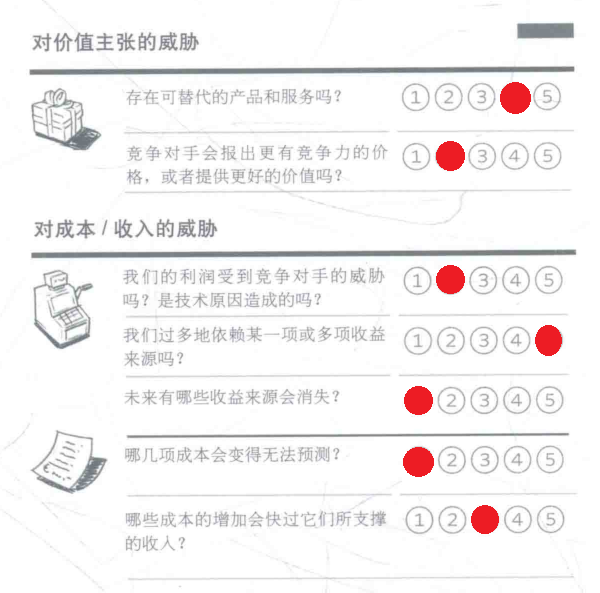
\includegraphics[width=15cm,height=15cm]{png/评估威胁}
    \end{figure}
    \clearpage % 强制图片开始新页面

    \subsubsection{价值主张评估}


    1.
    当前市场上确实存在有腾讯会议的代替产品。目前,在外国主流的视频会议软件,有 Skype 和后起之秀 Zoom,它们已经基本退出中国市场。
    而在国内,类似的视频会议软件,除了腾讯回忆,流行的还有钉钉、华为云会议、飞书等。
    虽然新冠疫情的流行对国内的视频会议市场进行了客观上的培养,使得腾讯会议得以借机迅速崛起,一举成为国内使用量最大的视频会议软件,
    \footnote{信息来源:https://www.iresearch.com.cn/Detail/report?id=3605\&isfree=0}
    但是不可否认,市场上仍有许多软件能提供腾讯会议所提供的产品和服务,这使得腾讯会议面临较大的被替代威胁


    2.
    腾讯会议的竞争对手不太能给出更有竞争力的价格,或供给更优质的服务。
    我们分别从华为云会议、钉钉、Zoom 以及腾讯会议的官方网站上获取了这些产品的报价和对应的功能。
    显而易见的是,这三中视频会议软件均采用了免费增值的商业模式,即均提供了含有基础功能的免费服务,和包含更高级功能、更强大性能的增值服务。
    华为云会议提供了250¥/月(3000¥/年)的标准版服务和350¥/月(4200¥/年)的旗舰版服务。
    \footnote{信息来源:https://www.huaweicloud.com/product/meeting.html}
    钉钉给出了最高的报价:9800¥/年的专业版服务、98000¥/年的专属版服务以及定制的专有版服务。
    \footnote{信息来源:https://pages.dingtalk.com/wow/z/tianyuan/default/opportunity\_index?spm=a213l2.13146415.0.0.7f1571e1F3EIGn}
    在国外流行的Zoom反而提出了远远低于上述软件的报价:149.90\$/年的专业版,199.90\$/年的商业版,以及更多的定制服务。但是,Zoom已经退出了中国市场,并不会对腾讯会议的国内市场造成威胁
    \footnote{信息来源:https://zoom.us/zh-cn/pricing}
    对比上述三家,腾讯会议的报价,面向个人的有 98¥/月(1176¥/年)、 499¥/月(5988¥/年)、999¥/月(11988¥/年),面向企业的有4788¥/年等报价,还有更多的版本可供选择,此处未列出。
    \footnote{信息来源:https://meeting.tencent.com/buy/index.html?mid=web.p.topdh.djygm}
    综上可以看出,腾讯会议提供了多种层次的不同价位服务,能满足各种层次需求的客户,其报价与功能与同行相比较也算适中,难以被同类产品从价格和价值方面威胁。


    \subsubsection{成本/收入评估}
    1.
    腾讯会议的利润几乎不会受到竞争对手的威胁。其原因在价值主张评估中已经提到:腾讯会议在新冠疫情发生后,迅速占领了国内市场的大量份额,一跃成为国内的主流视频会议软件。
    除非再发生一次类似新冠疫情的事件培养出更大的行业市场,或者行业中有革命性的软件出现,否则腾讯会议的营收很难被其他同类软件抢走。
    值得一提的是,腾讯会议是属于腾讯的产品,而腾讯旗下还有微信、QQ等被国民普遍使用的应用。腾讯会议依靠腾讯庞大的资金量、技术库、应用生态链和用户数量,是较难被同类产品威胁到利润的。


    2.
    腾讯会议依赖单一的收入来源,即增值服务。
    我们从腾讯的2022年度报表中,可以看出增值服务是腾讯的主要收入来源,其占总收入的百分比为52\%,而金融科技及企业服务占31\%,广告仅收入占16\%。
    \footnote{信息来源:https://static.www.tencent.com/uploads/2023/04/06/eac54c79c67d8a501bc4b65ff1718223.pdf}
    一方面,当今的商业办公软件注重于提高用户的办公效率而很少有投放广告的。
    腾讯会议本身的办公软件性质决定了腾讯几乎不可能在腾讯会议投放娱乐广告以营收,这会降低腾讯会议的商务性和严肃性,在市场上仍有大量可替代产品的情况下,此举很可能造成用户的流失和增值服务收入的减少。
    腾讯会议也绝不能收集会议信息以定向投放广告,因为窃听会议会严重侵犯其他组织的机密。
    也就是说,作为服务办公场景人群的软件,腾讯会议至多能投放少量的商务办公软件广告以获得少量的广告收入。
    另一方面,腾讯会议与金融科技无关,同时软件本身又必然要追求简单易用以吸引用户,因而不太可能依靠向企业提供技术支持等服务来营收。
    因此,增值服务几乎就是腾讯会议唯一所能依靠的收入来源。


    3.
    腾讯会议未来可能会出现收益缩减,但不会出现收益来源会消失的情景。
    其原因也在上述分析中提到过:腾讯会议是免费增值的商业模式,依靠增值服务作为唯一收益来源。
    在这种情况下,腾讯会议的收益缩减主要有两种可能:
    一是市场产生一定程度的萎缩,导致收益减少,市场萎缩可能来源于随着疫情的消失等因素;
    二是市场上出现价格更低、服务更好、价值更高的同类替代产品,或是有革命性的新产品出现,抢占腾讯会议市场份额。
    第一种情况,从以上 iResearch 的调查报告中我们也可以看到腾讯会议的下载量在后疫情时代确实有所下降。
    第二种情况,我们已经知道腾讯会议有较多的同类替代产品,却鲜有能给出更高性价比而抢走份额的产品。
    综上,增值收费作为腾讯会议近乎唯一的收入来源,在近未来可能会有所缩减,但几乎不可能会消失,因为一旦消失就意味着腾讯会议这个产品彻底失败


    4.
    腾讯会议发展至今,已经几乎没有可不预测的成本了。
    腾讯会议早已开发完毕,开发成本已然确定;
    进入稳定部署维护的阶段已经历较长时间,已然度过了疫情初期的使用高峰,对于维护平台正常运行所需要的核心设备资源和人员成本都已经有了数据。
    不出意外的话,腾讯会议不会再遇到不可预测的成本。

    5.
    腾讯会议的运维成本可能迅速增大,超过腾讯会议所能提供的增值服务收入。
    一个现实例子是,在疫情爆发后,线上办公需求井喷式增长。根据腾讯科技讯介绍,腾讯会议为满足市场需求,在8天内增加了逾10万台云主机,超过100万核的计算资源。
    \footnote{信息来源:https://new.qq.com/rain/a/TEC2020020600971700}
    然而在当时,或许是出于抢占市场份额的目的,腾讯会议并没有急于收取增值服务费用,而是向大众免费提供了高质量的视频会议服务。
    这样的策略,一方面确实为腾讯会议吸引了大量的用户,但却没有带来收入;另一方面,用户数量的剧增使得腾讯会议的运维成本也随之剧增。
    由于腾讯并没有公布腾讯会议的成本收入数据,我们并不能直接得出腾讯会议的成本超过收入的结论。
    但是,观察同类产品 Zoom 在同一时间段的利润表,我可以发现 Zoom 在当时的利润率仅有 3\%。
    \footnote{信息来源:https://quotes.sina.com.cn/usstock/hq/income.php?s=zm\&t=annual}
    由此,我们可以推测,腾讯会议当时在短时间内的运维成本迅速增加,却没能像 Zoom 那样收取到增值服务营收,其结果就是腾讯会议的运营成本超过了腾讯会议所能带来的收入。
    也许这种成本超过收入的情况再次发生的概率不大,但确实存在这种潜在威胁。

    \subsection{评估机会}\label{subsec:opportunity}
    \subsubsection{打分结果}
    \begin{figure}[htbp]
        \centering
        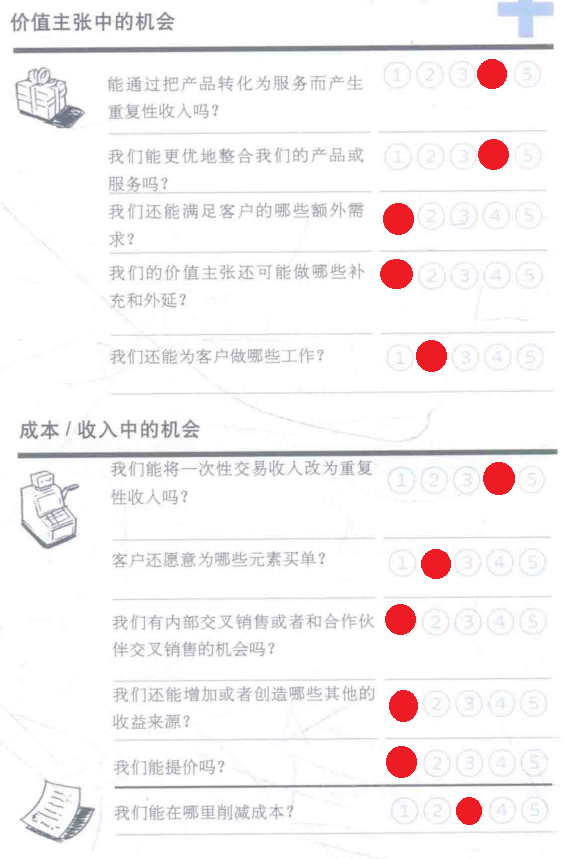
\includegraphics[width=12cm,height=18cm]{png/评估机会}
    \end{figure}
    \clearpage % 强制图片开始新页面


    \subsubsection{价值主张评估}


    1.
    我们已经在评估威胁中分析腾讯会议定价时论述过,腾讯会议并不是买断式的软件产品,而是采用月租、年租的形式收取增值服务的租金。
    事实上,腾讯会议还提供了所谓的“腾讯会议 SaaS 版新购”的服务购买方式。
    \footnote{信息来源:https://buy.cloud.tencent.com/tm}
    显然我们可以得出结论: 腾讯会议已然是通过提供服务的方式获取重复性收入。


    2.
    在整合产品和服务方面,腾讯确实还有改进空间。
    同样我们已经分析过,腾讯会议借助QQ、微信等腾讯下属的应用生态链迅速占领了市场。
    实际上,腾讯还可以做得更好。理由是,腾讯会议可以通过QQ、微信账号进行登录,产品之间进行了一定程度的整合。
    但腾讯还可以更进一步整合产品和服务,例如将腾讯会议等产品的入口嵌入QQ、微信等腾讯旗下的其他产品中,形成一个联系更紧、整合程度更深的应用生态链,将QQ、微信上的庞大用户群引向腾讯会议,
    这样不仅能方便用户享受腾讯的服务体系,更能凭借巨大的用户基数牢牢地占领视频会议软件的市场。


    3.
    我们认为,基本已经没有额外的客户需求可供腾讯会议发掘。
    除了基本的视频会议服务,腾讯会议还提供了包括共享桌面、文字图片聊天室、AI识别等各方面的额外服务。
    也就是说,腾讯会议与在线会议有关的服务已经趋于全面,客服需求基本发掘完毕。
    假如强行添加更多功能,反而既增加了成本,又使得应用变得冗余臃肿,结果是吃力不讨好。


    4.
    腾讯会议的价值主张目前已经基本没有补充和外延的机会。
    正如我们在 4.3.2.3 中的分析所说,腾讯会议应该专注于在线会议的价值主张,提高客户的办公效率,而非盲目延展价值主张造成软件的臃肿。


    5.
    尽管我们认为腾讯会议的价值主张基本没有横向扩展的空间了,但腾讯会议仍可以在已有价值主张方面提供更优质的服务。
    例如,腾讯会议可以优化性能,通过提高网络吞吐量、降低硬件占用率等措施提高用户的使用体验。
    腾讯会议还提供了语音识别服务,自动从数小时的会议音视频录制文件中识别语言并提供字幕,而字幕也是提高用户使用体验的重要方面。
    不过,在语音识别方面,腾讯会议的识别能力也有改进空间。
    综上,腾讯会议还有进一步优化已有功能以提高客户使用体验的空间。


    \subsubsection{成本/收入评估}


    1.
    腾讯会议的重复性收入问题我们已进行详细的讨论,请见 4.3.2.1。


    2.
    在评估价值主张的机会评估中我们提及,假如腾讯会议能深度优化应用以提高应用体验,特别是更好的AI服务,或许能吸引更多的用户买单。
    目前腾讯会议的 AI 已经做到了自动为会议做分段、概括、语音识别,尽管其精确度仍有待提高,但确实为用户提供了很大便利。
    在线会议的效果越接近面对面会议,就越能吸引更多用户买单。


    3.
    腾讯会议内部销售及向合作伙伴销售的意义不大。
    腾讯会议的最大“合作伙伴”就是腾讯公司内部的其他部门。
    腾讯内部的会议需求,大部分都可以通过面对面会议解决,当确实有远程需求时也应该免费向员工提供腾讯会议服务。
    由企业内其他部门和员工为本公司开发的生产工具买单是荒诞的行为。


    4.
    正如我们已经说过的,增值服务是腾讯会议的最主要的收入来源,也应当是最主要的收入来源。
    腾讯会议应该把目光集中在增值服务收入上,而不应该聚焦于广告、技术支持等其他收入。


    5.
    腾讯会议提价的空间不大。
    在市场上仍存在很多替代产品,且客户可以转向线下会议的情况下,腾讯会议再提价很可能造成客户流失,反而可能造成总收入下降。
    在市场均价没有上升之前,或腾讯会议没有大幅由于其他产品之前,对于提价行为必须十分谨慎。

    6.
    腾讯会议确实有不少的降低成本空间。
    我们前文提过,腾讯会议的主要成本在于大量的算力资源成本和运维成本。
    优化算法、优化代码结构、适当减少向免费用户提供的服务、删减不必要的服务等方式,都有可能降低运维成本。

    \section{蓝海战略}
    

\section{更新过的商业模式画布}


    
\end{document}
